\documentclass[11pt]{article}

%==============Packages & Commands==============
\usepackage{graphicx}
\usepackage{fancyvrb}
\usepackage{tikz}
%%%<
\usepackage{verbatim}
%\usepackage[active,tightpage]{preview}
%\PreviewEnvironment{tikzpicture}
%\setlength\PreviewBorder{5pt}%

\usepackage{geometry}                		% See geometry.pdf to learn the layout options. There are lots.
% \geometry{a4paper}                   		% ... or a4paper or a5paper or ...
%\geometry{landscape}                		% Activat\usetikzlibrary{arrows}e for for rotated page geometry
%\usepackage[parfill]{parskip}    		% Activate to begin paragraphs with an empty line rather than an indent
\usepackage{graphicx}				% Use pdf, png, jpg, or eps§ with pdflatex; use eps in DVI mode
								% TeX will automatically convert eps --> pdf in pdflatex
\usepackage{amssymb}

\usepackage[ruled,vlined]{algorithm2e}
\usetikzlibrary{arrows}
\usepackage{alltt}
\usepackage[T1]{fontenc}
\usepackage[utf8]{inputenc}
\usepackage{indentfirst}
\usepackage[longnamesfirst]{natbib} % For references
\bibpunct{(}{)}{;}{a}{}{,} % Reference punctuation
\usepackage{changepage}
\usepackage{setspace}
\usepackage{booktabs} % For tables
\usepackage{rotating} % For sideways tables/figures
\usepackage{amsmath}
\usepackage{multirow}
\usepackage{color}
\usepackage{dcolumn}
\usepackage{comment}
%\usepackage{fullwidth}
\newcolumntype{d}[1]{D{.}{\cdot}{#1}}
\newcolumntype{.}{D{.}{.}{-1}}
\newcolumntype{3}{D{.}{.}{3}}
\newcolumntype{4}{D{.}{.}{4}}
\newcolumntype{5}{D{.}{.}{5}}
\usepackage{float}
\usepackage[hyphens]{url}
%\usepackage[margin = 1.25in]{geometry}
%\usepackage[nolists,figuresfirst]{endfloat} % Figures and tables at the end
\usepackage{subfig}
\captionsetup[subfloat]{position = top, font = normalsize} % For sub-figure captions
\usepackage{fancyhdr}
%\makeatletter
%\def\url@leostyle{%
%  \@ifundefined{selectfont}{\def\UrlFont{\sf}}{\def\UrlFont{\small\ttfamily}}}
%\makeatother
%% Now actually use the newly defined style.
\urlstyle{same}
\usepackage{times}

\usepackage{lscape}
% \usepackage{mathptmx}
%\usepackage[colorlinks = true,
%						bookmarksopen = true,
%						pagebackref = true,
%						linkcolor = black,
%						citecolor = black,
% 					urlcolor = black]{hyperref}
%\usepackage[all]{hypcap}
%\urlstyle{same}
\newcommand{\fnote}[1]{\footnote{\normalsize{#1}}} % 12 pt, double spaced footnotes
\def\citeapos#1{\citeauthor{#1}'s (\citeyear{#1})}
\def\citeaposs#1{\citeauthor{#1}' (\citeyear{#1})}
\newcommand{\bm}[1]{\boldsymbol{#1}} %makes bold math symbols easier
\newcommand{\R}{\textsf{R}\space} %R in textsf font
\newcommand{\netinf}{\texttt{NetInf}\space} %R in textsf font
\newcommand{\iid}{i.i.d} %shorthand for iid
\newcommand{\cites}{{\bf \textcolor{red}{CITES}}} %shorthand for iid
%\usepackage[compact]{titlesec}
%\titlespacing{\section}{0pt}{*0}{*0}
%\titlespacing{\subsection}{0pt}{*0}{*0}
%\titlespacing{\subsubsection}{0pt}{*0}{*0}
%\setlength{\parskip}{0pt}
%\setlength{\parsep}{0pt}
%\setlength{\bibsep}{2pt}
%\renewcommand{\headrulewidth}{0pt}

%\renewcommand{\figureplace}{ % This places [Insert Table X here] and [Insert Figure Y here] in the text
%\begin{center}
%[Insert \figurename~\thepostfig\ here]
%\end{center}}
%\renewcommand{\tableplace}{%
%\begin{center}
%[Insert \tablename~\theposttbl\ here]
%\end{center}}

\newcommand\independent{\protect\mathpalette{\protect\independenT}{\perp}}
\def\independenT#1#2{\mathrel{\rlap{$#1#2$}\mkern2mu{#1#2}}}
\newcommand{\N}{\mathcal{N}}
\newcommand{\Y}{\bm{\mathcal{Y}}}
\newcommand{\bZ}{\bm{Z}}

\usepackage[colorlinks = TRUE, urlcolor = black, linkcolor = black, citecolor = black, pdfstartview = FitV]{hyperref}


%============Article Title, Authors==================
\title{\vspace{-2cm} The effects of transitions of power on the contents of municipal government websites }


\author{ Markus Neumann \and Bruce Desmarais \and Hanna Wallach} \date{\today}



%===================Startup=======================
\begin{document}
\maketitle



%=============Abstract & Keywords==================

\begin{abstract}

\noindent We explore the effect of transitions of power in municipal governments on the content of their websites. We hypothesize that when party control changes, city administrators modify the contents of their websites in order to fit the agenda of the new incumbent. To test this theory, we study cities in Indiana and Louisiana, two states in which all municipal elections are partisan and the parties of the candidates appear on the ballots. Snapshots of websites before and after transitions of power are acquired through the Wayback Machine. We apply statistical topic models based in latent dirichlet allocation, focusing on changes to the websites. We present results on both which topics see the greatest degree of change associated with transitions in city administrations, and how the topics modified differ with regard to political parties.

\end{abstract}
\thispagestyle{empty}
% \doublespacing
% Description of the possible challenges
\section{Introduction}

\section{Background}

\cite{grimmelikhuijsen2010transparency} run an experiment in which citizens are exposed to randomly selected levels of information about local government council minutes. They find a negative relationship between the information level and perceptions of competence in the local government. This raises an interesting question regarding whether citizens or more likely to participate when they perceive competence or when they perceive incompetence.

\cite{wang2005evaluating} present a widely cited `model' for evaluating the accessibility of information on government websites. This is an important paper with which we should be familiar at a very detailed level as we use archived web content to assess the volume/accessibility of information provided by local governments.

\cite{osman2014cobra} is less relevant, but they develop a multi-item measure to predict the level of citizen satisfaction with e-government services. 


\cite{grimmelikhuijsen2012developing} conduct an enormously relevant study. Insofar as we analyze what predicts openness of government websites, we will be replicating and building upon this study. They focus on Dutch municipal websites, and their approach is fairly limited in scope and highly manual (which we can compliment). For example, one of the dependent variables ``Decision-making transparency,'' is measured ``using a discrete (1/0) indicator for whether the underlying principles or reasons for local air pollution policies were given on the Web site.'' 

\begin{landscape}
\begin{table}[htbp]
	%\caption{}
	\begin{tabular}{|p{2cm}|c|p{3cm}|p{12cm}|l|}
		\hline
		Names & Year & Journal & Findings & Important? \\ \hline
		Benedictis-Kessner, Justin De
		Warshaw, Christopher & 2016 & JOP* & Regression discontinuity design. Democratic mayors spend more (but it is unclear on what, not the typical Democratic issue-areas), issue more debt, pay more interest & Yes \\ \hline
		Caughey, Devin
		Warshaw, Christopher
		Xu, Yiqing & 2015 & Working Paper & Regression discontinuity design. Partisan composition of state governments affects state policy liberalism (composite index for the areas of social welfare, taxation, labor, civil rights, women’s rights, moral legislation, family planning, environment). & Somewhat \\ \hline
		Einstein, Katherine Levine
		Kogan, Vladimir & 2015 & Urban Affairs Review & Cities with more Democratic citizens spend more; more progressive (rather than regressive) forms of taxation; pursue intergov. aid more; spend more on police, fire, parks \& recreation & Somewhat \\ \hline
		Einstein, Katherine Levine
		Glick, David M. & 2015 & Working Paper & Survey of 72 mayors. Unlike Republican mayors, roughly half of Democrats seem to agree that cities should aim to reduce inequality. Democratic mayors also seem to favor redistribution to accomplish that goal. & Somewhat \\ \hline
		Kiewiet, D Roderick
		Mccubbins, Mathew D & 2014 & Annual Review & City budgets have been severeley constrained since the Great Recession. Spending has thus decreased in general. Lack of funds means that there is not much discretion for partisanship. & Somewhat \\ \hline
		Tausanovitch, Chris
		Warshaw, Christopher & 2014 & APSR* & Cities are responsive (taxes, expenditures, regressiveness of taxation) to citizens' conservatism/liberalism. Partisan elections do not make cities more or less responsive. & Yes \\ \hline
		Guillamón, Ma Dolores
		Bastida, Francisco
		Benito, Bernardino & 2013 & European Journal of Law and Economics & Police spending in Spain. Conservative parties spend more on police. Spending is higher before elections. Also contains a useful overview of the literature. & Yes \\ \hline
	\end{tabular}
	\label{}
\end{table}
\end{landscape}

\begin{landscape}
	\begin{table}[htbp]
		%\caption{}
		\begin{tabular}{|p{2cm}|c|p{3cm}|p{12cm}|l|}
			\hline
			Gerber, Elisabeth R. & 2013 & Cityscape & Partisanship of both citizens and elected city officials separately affect climate policy. & Yes \\ \hline
			Names & Year & Journal & Findings & Important? \\ \hline
			Solé-Ollé, Albert
			Viladecans-Marsal, Elisabet & 2013 & Journal of Urban Economics & Spanish cities. The authors "employ a regression discontinuity design to document that cities controlled by left-wing parties convert much less land from rural to urban uses than is the case in similar cities con- trolled by the right". Partisanship might also affect housing construction and price growth. & Yes \\ \hline
			Gerber, Elisabeth R.
			Hopkins, Daniel J. & 2011 & AJPS & Regression discontinuity design. Democratic mayors spend less on public safety. All other policy areas (including taxation) are unaffected. & Yes \\ \hline
			Trounstine, Jessica & 2010 & Annual Review & Race and ethnicity in local elections (not relevant to us). Partisan elections have higher turnout; non-partisan elections still tend to have some partisanship in them because voters learn about party of candidates from media. Non-partisan elections favor Republicans/upper class. Mixed evidence for whether partisanship of mayor is important for policy. & Somewhat \\ \hline
			Palus, Christine Kelleher & 2010 & State and Local Government Review & Ideology (liberal/conservative) of citizen is well represented by gov. spending in five areas: (1) community development, housing, and conservation, (2) health and human services, (3) culture, the arts, and recreation, (4) environmental programs, and (5) transportation. & Somewhat \\ \hline
			Ferreira, Fernando
			Gyourko, Joseph & 2009 & The Quarterly Journal of Economics & Regression discontinuity design. Null results for spending and city gov. size with regard to mayor partisanship. & Yes \\ \hline
			Ansolabehere, Stephen
			Snyder, James M. & 2006 & Scandinavian Journal of Economics & Despite the journal, this is about the U.S. The important finding (for us) is the fact that counties whose government is controlled by the same party as the state government, receive more funding (county's share of state transfers, normalized by county pop.) from the state. & Somewhat \\ \hline
			Murphy, Russell D. & 2002 & Annual Review & Not useful. Too philosophical; mostly cites papers written a hundred years ago. Also exclusively about larger cities. & No \\ \hline
		\end{tabular}
		\label{}
	\end{table}
\end{landscape}

There doesn't seem to be much literature on transitions of party control, if anything, that question is mostly phrased with regard to political representation. However, if we want to tie our paper to a larger theory, we could go with dynamic representation. Under dynamic representation, policy-makers are responsive to trends in citizens opinions, which mainly manifest/become apparent through election results, especially when incumbents are voted out of office. This fits our topic quite well. Also, of the few papers that do exist on the effects of partisan transitions, virtually all use regression discontinuity designs.

\section{Data}
The General Services Administration (GSA) maintains all .gov addresses, and provides a complete\footnote{Domains used for testing and internal programs are excluded.} list of all such domains to the public through GitHub\footnote{https://github.com/GSA/data/tree/gh-pages/dotgov-domains}. This list is updated once per month - we rely on the version released on January 16, 2017. The data from the GSA contains the following variables: One, domain name, specifically, the all-uppercase version of domain and top-level domain (for example, 'ABERDEENMD.GOV'). Two, the type of government entity to which the domain is registered, such as city, county, federal agency, etc. Three, for federal agencies, the name is specfied. Finally, the city in which the domain is registered, is noted.

Here, we focus only on cities. As a first step, we use a webdriver-controlled browser (Firefox/Selenium/Geckodriver) to test whether all of the city websites actually work. Of the 2425 domains listed by the GSA as cities, 292 are not accessible. Furthermore, the .gov domain, as registered at the GSA, is frequently not the website a city actually uses. In many cases, these sites redirect to another address, sometimes not a .gov domain (in this case, we simply use this domain). We record these URLs, as they are required to retrieve the images websites stored in the Wayback Machine (WbM).

In order to provide an overview of our coverage (as not all cities, towns and villages use .gov addresses), we merge this list with U.S. Census data\footnote{http://www2.census.gov/programs-surveys/popest/datasets/2010-2015/cities/totals/sub-est2015\_all.csv}. Here, several limitations in the GSA data need to be accounted for: One, even though the GSA nominally separates websites of cities and counties, some of the domains categorized as cities actually belong to counties. The same is true for townships and boroughs. Ergo, we eliminate all websites belonging to these three types of entities by hand. Furthermore, the city name, as given by the GSA, refers to the city in which the domain is registered, which is not necessarily equivalent to the city the website serves. In many cases, a website of a larger city may be registered to one of its subdivisions (for example, the website of New York is registered to Brooklyn), or vice versa (for example, the website of Homecroftin, a small town within Indianapolis, is registered to the city as a whole). Consequently we fix mismatches between websites and cities manually. Finally, a number of cities are simply misspelled, which we also correct by hand.

After the counties, townships and cities that cannot be matched to the Census data\footnote{There are five cities that are not contained in the Census data} and duplicate websites (some cities have more than one website) are removed, 1813 domains/cities remain.

These cities contain 90,616,865 people, and thus about 28\% of the U.S. population (see figure 1).

\begin{figure}[!ht]
	\centering
	%\caption{Population coverage}
	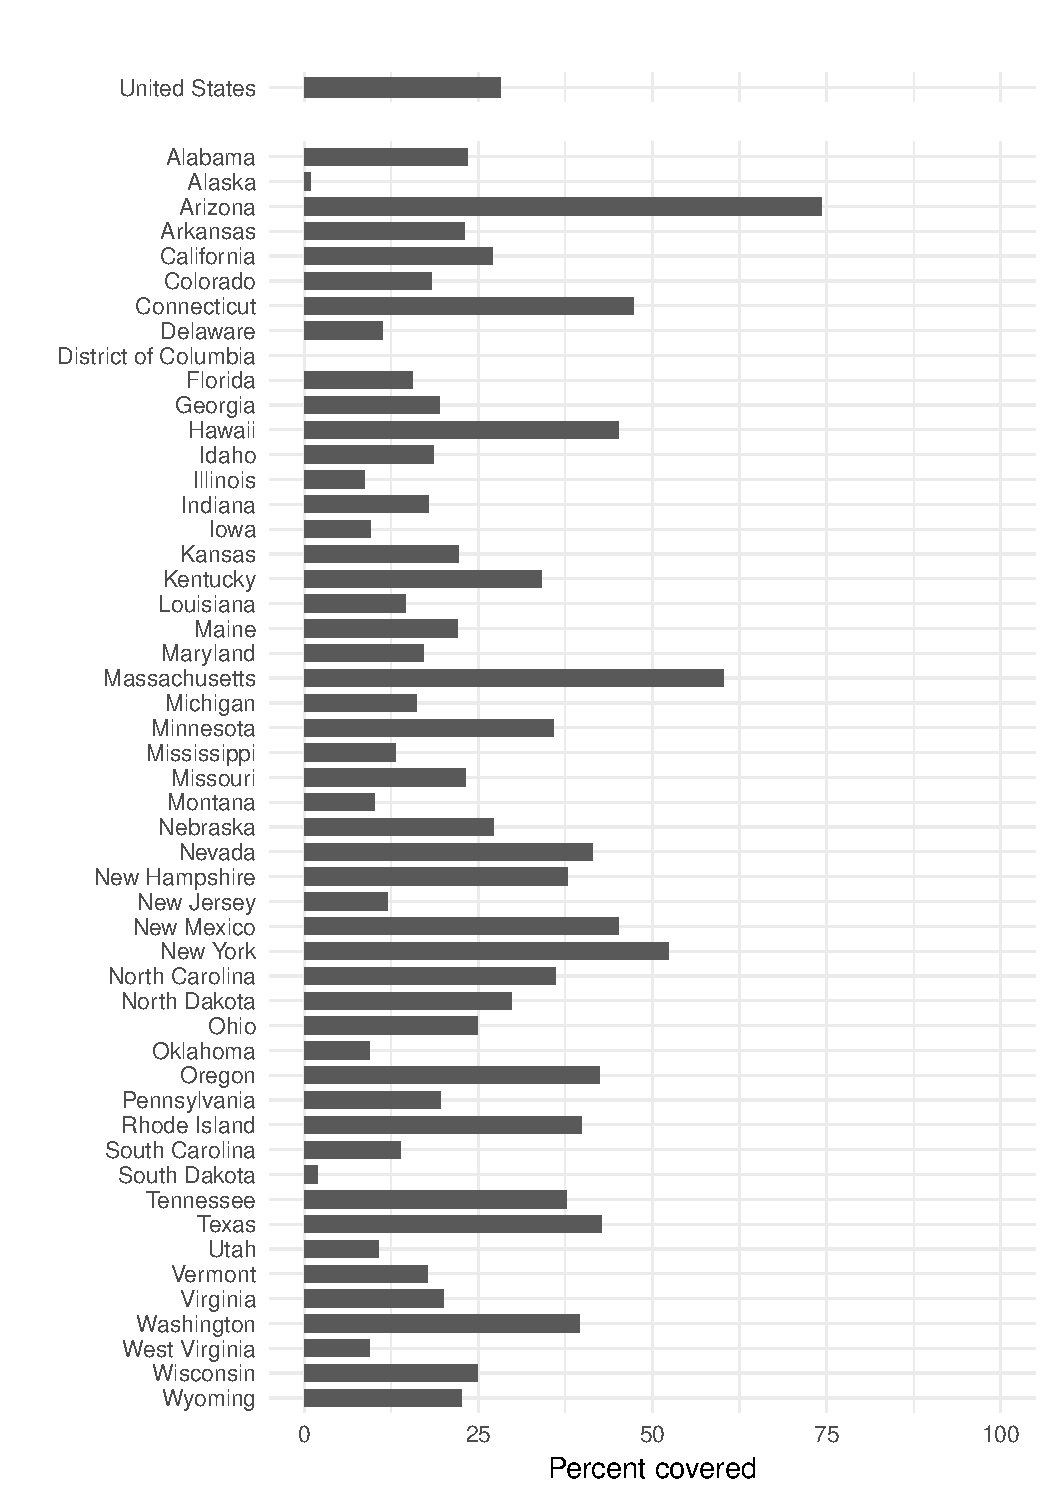
\includegraphics[width=0.9\linewidth,height=0.9\textheight]{figures/coverage_states.pdf}
\end{figure}

We use the resulting list of websites to acccess their copies stored in the Internet Archive's Wayback Machine. To this end, we rely on the Ruby Gem 'Wayback Machine Downloader'\footnote{https://github.com/hartator/wayback-machine-downloader} (WbMD). We supply the URL that each .gov website redirects to to the WbMD, which then downloads every file present in the WbM from a snapshot in October 2016, or, if not available, as soon as possible after this point.

<Note: We have not actually done this last step for all websites (however, the R script which runs the Ruby package is already set up to do so once we need to). Instead 10 websites were randomly sampled from an older version of the GSA list, which still contained counties and townships, which is why one of the 10 websites is from Dutchess County, NY.>

% latex table generated in R 3.4.0 by xtable 1.8-2 package
% Tue May 23 19:28:26 2017
\begin{table}[ht]
	\centering
	\begin{tabular}{lrrr}
		\hline
		Filetype & current & before & after \\ 
		\hline
		& 51455 & 13866 & 19199 \\ 
		pdf & 9646 & 5489 & 7544 \\ 
		jpg & 5216 & 1988 & 3512 \\ 
		html & 3767 & 17842 & 17596 \\ 
		aspx & 2832 & 4356 & 3271 \\ 
		png & 2714 & 2327 & 3684 \\ 
		gif & 1068 & 664 & 1077 \\ 
		JPG & 478 & 182 & 263 \\ 
		1 & 443 &  61 &  54 \\ 
		css & 390 & 265 & 518 \\ 
		js & 350 & 255 & 468 \\ 
		htm & 264 & 295 & 256 \\ 
		docx & 203 & 106 & 120 \\ 
		doc & 167 &  70 & 130 \\ 
		asp & 161 & 201 & 211 \\ 
		svg &  87 &  55 &  69 \\ 
		php &  83 & 157 & 241 \\ 
		\hline
	\end{tabular}
	\caption{The most common file types in scraped websites} 
\end{table}

\begin{landscape}
% latex table generated in R 3.4.0 by xtable 1.8-2 package
% Tue May 23 19:35:22 2017
\begin{table}[ht]
	\centering
	\footnotesize
	\begin{tabular}{lrrrrrrrrr}
		\hline
		Website & current\_size & current\_files & before\_size & before\_files & after\_size & after\_files & size\_change & files\_change & control\_change \\ 
		\hline
		attica-in.gov & 61988 & 1417 & 7528 & 164 & 55956 & 1390 & 7.43 & 8.48 & 0.00 \\ 
		bedford.in.us & 57628 & 560 & 27452 & 182 & 46388 & 525 & 1.69 & 2.88 & 0.00 \\ 
		cityofboonvilleindiana.com & 9848 & 110 & 16996 & 172 & 20784 & 229 & 1.22 & 1.33 & 0.00 \\ 
		frankfort-in.gov & 205368 & 2652 & 12208 & 242 & 138360 & 1077 & 11.33 & 4.45 & 0.00 \\ 
		warsaw.in.gov & 298440 & 2117 & 26844 & 539 & 360400 & 2036 & 13.43 & 3.78 & 0.00 \\ 
		www.bloomington.in.gov & 131128 & 2713 & 443360 & 14384 & 247096 & 9640 & 0.56 & 0.67 & 0.00 \\ 
		www.brazil.in.gov & 43056 & 845 & 34472 & 625 & 55152 & 1214 & 1.60 & 1.94 & 0.00 \\ 
		www.carmel.in.gov & 2270016 & 8727 & 1919344 & 5361 & 899900 & 2219 & 0.47 & 0.41 & 0.00 \\ 
		www.ci.auburn.in.us & 183296 & 1025 & 21444 & 345 & 23564 & 211 & 1.10 & 0.61 & 0.00 \\ 
		www.cityoffortwayne.org & 2136424 & 4378 & 266784 & 3582 & 233600 & 3018 & 0.88 & 0.84 & 0.00 \\ 
		www.cityofhobart.org & 722000 & 2463 & 44192 & 650 & 62660 & 1037 & 1.42 & 1.60 & 0.00 \\ 
		www.evansvillegov.org & 6345932 & 11844 & 290784 & 1281 & 1697224 & 6853 & 5.84 & 5.35 & 0.00 \\ 
		www.gary.in.us & 373888 & 1227 & 121812 & 485 & 157140 & 719 & 1.29 & 1.48 & 0.00 \\ 
		www.huntingburg-in.gov & 388680 & 2496 & 8644 & 213 & 375900 & 1953 & 43.49 & 9.17 & 0.00 \\ 
		www.jasperindiana.gov & 561968 & 4013 & 55900 & 460 & 439072 & 2224 & 7.85 & 4.83 & 0.00 \\ 
		www.lakestation-in.gov &  48 &   2 & 7724 &  84 & 257272 & 1097 & 33.31 & 13.06 & 0.00 \\ 
		www.linton-in.gov &  32 &   1 &  24 &   2 &  24 &   2 & 1.00 & 1.00 & 0.00 \\ 
		www.madison-in.gov & 531044 & 1848 & 36636 & 575 & 191624 & 1444 & 5.23 & 2.51 & 0.00 \\ 
		www.martinsville.in.gov & 46792 & 1463 & 71628 & 1052 & 80944 & 800 & 1.13 & 0.76 & 0.00 \\ 
		www.monticelloin.gov & 33656 & 753 & 18120 & 448 & 100680 & 2104 & 5.56 & 4.70 & 0.00 \\ 
		www.newhavenin.org & 84364 & 626 & 2524 &  86 & 6792 & 334 & 2.69 & 3.88 & 0.00 \\ 
		www.richmondindiana.gov & 250968 & 1042 & 217252 & 918 & 401672 & 2422 & 1.85 & 2.64 & 0.00 \\ 
		www.southbendin.gov & 1264076 & 4749 & 454456 & 3286 & 1424136 & 2562 & 3.13 & 0.78 & 0.00 \\ 
		connersvillecommunity.com & 170688 & 569 & 162316 & 815 & 187276 & 808 & 1.15 & 0.99 & 1.00 \\ 
		www.batesvilleindiana.us & 166564 & 2348 & 39592 & 496 & 95696 & 1310 & 2.42 & 2.64 & 1.00 \\ 
		www.cityofrisingsun.com & 994956 & 3311 & 321400 & 1268 & 80848 & 868 & 0.25 & 0.68 & 1.00 \\ 
		www.cityofrockport-in.gov & 12068 &  98 & 5148 &  16 & 12068 &  98 & 2.34 & 6.12 & 1.00 \\ 
		www.elkhartindiana.org & 1132828 & 2345 & 5588 & 123 & 6204 & 223 & 1.11 & 1.81 & 1.00 \\ 
		www.elwoodcity-in.org & 224412 & 765 & 5000 & 123 & 139692 & 517 & 27.94 & 4.20 & 1.00 \\ 
		www.indy.gov & 5726048 & 9675 & 6119260 & 10451 & 4984080 & 7981 & 0.81 & 0.76 & 1.00 \\ 
		www.northvernon-in.gov & 272016 & 403 & 3132 & 112 & 289336 & 416 & 92.38 & 3.71 & 1.00 \\ 
		www.winchester-in.gov & 364592 & 2480 & 6508 & 135 & 45488 & 567 & 6.99 & 4.20 & 1.00 \\ 
		\hline
	\end{tabular}
	\caption{Number of files and size of websites} 
\end{table}
\end{landscape}

% latex table generated in R 3.3.2 by xtable 1.8-2 package
% Wed Mar  1 11:55:24 2017
\begin{table}[ht]
	\centering
	\begin{tabular}{rr}
		\hline
		& tf \\ 
		\hline
		tax & 176324 \\ 
		date & 98949 \\ 
		due & 97192 \\ 
		amt & 96382 \\ 
		town & 86726 \\ 
		value & 81119 \\ 
		total & 70825 \\ 
		parcel & 63589 \\ 
		county & 56201 \\ 
		market & 51758 \\ 
		east & 51357 \\ 
		full & 51199 \\ 
		nrth & 50566 \\ 
		book & 50306 \\ 
		deed & 50231 \\ 
		bill & 49719 \\ 
		acres & 48935 \\ 
		acct & 44871 \\ 
		csd & 43792 \\ 
		owners & 43510 \\ 
		res & 41803 \\ 
		family & 36883 \\ 
		fire & 35156 \\ 
		school & 33685 \\ 
		name & 30382 \\ 
		red & 30362 \\ 
		taxable & 30248 \\ 
		hook & 29902 \\ 
		homestead & 29287 \\ 
		outside & 28593 \\ 
		\hline
	\end{tabular}
	\caption{Top term frequencies for 10 test websites} 
\end{table}

\subsection{Indiana City Websites}

It would be fine to focus on Indiana as a case. First, we need to answer some preliminary questions about the data.

\begin{enumerate}

\item For what percentage and number of IN cities can we find data from the WBM?
\item For how many election cycles can we find political leadership data for these matched cities?
\item In what number and percentage of cities is the local leadership majority Republican? 
\item Relatedly, in a typical election cycle, for how many cities do we see a transition in party leadership (i.e., a shift from majority D (R) to majority (R) D). 

\end{enumerate}

\begin{enumerate}
	
	\item 30 cities, with a combined population of 1,180,435. However, since only cities (as opposed to towns and villages) hold mayoral elections, only 16 of these, with a combined population of 1,094,383 can be matched to the election data.
	\item 2015, 2011, 2007, 2003.
	\item Of the 16 cities, 7 have Republican mayors after the 2015 elections.
	\item In 6 cases, a shift of party control occurs, with 4 of these being Republican --> Democratic. 
	
\end{enumerate}

% latex table generated in R 3.3.3 by xtable 1.8-2 package
% Wed Mar 22 11:32:43 2017
\begin{table}[ht]
	\centering
	\begin{tabular}{lrrlrrl}
		\hline
		City & DemVotes & RepVotes & Winner & Change & Pop15 & url \\ 
		\hline
		Attica &  & 187 & Republican & 0 & 3117 & https://attica-in.gov/ \\ 
		Connersville & 1005 & 995 & Democratic & 1 & 13010 & http://connersvillecommunity.com/ \\ 
		Frankfort &  & 1748 & Republican & 0 & 16060 & http://frankfort-in.gov/ \\ 
		Huntingburg & 447 & 793 & Republican & 0 & 6035 & http://www.huntingburg-in.gov/ \\ 
		Indianapolis & 92830 & 56661 & Democratic & 1 & 862781 & http://www.indy.gov \\ 
		Lake Station & 1483 & 227 & Democratic & 0 & 12054 & http://www.lakestation-in.gov/ \\ 
		Linton & 785 & 692 & Democratic & 0 & 5284 & http://www.linton-in.gov/ \\ 
		Madison & 1192 & 1915 & Republican & 0 & 12040 & http://www.madison-in.gov/ \\ 
		Mitchell & 229 & 495 & Republican & 1 & 4252 & http://mitchell-in.com/ \\ 
		Monticello & 0 &  & Democratic & 0 & 5322 & http://www.monticelloin.gov/ \\ 
		North Vernon & 679 & 697 & Republican & 1 & 6619 & http://www.northvernon-in.gov/ \\ 
		Richmond & 3421 & 2731 & Democratic & 0 & 35854 & http://www.richmondindiana.gov/ \\ 
		Rockport & 286 & 272 & Democratic & 1 & 2223 & http://www.cityofrockport-in.gov/ \\ 
		South Bend & 8515 & 2074 & Democratic & 0 & 101516 & https://www.southbendin.gov/ \\ 
		Union City & 338 & 440 & Republican & 0 & 3447 & http://www.unioncity-in.gov/ \\ 
		Winchester & 606 & 524 & Democratic & 1 & 4769 & http://www.winchester-in.gov/ \\ 
		\hline
	\end{tabular}
	\caption{} 
\end{table}

\subsection{Research Design}

\begin{table}[ht]
	\centering
	\begin{tabular}{llr}
		\hline
		Variable & Unit & Source \\
		\hline
		Population size & 1000 people & Census \\
		Population growth last 5 years & Percent & Census \\
		Type of economy (agriculture/industry/services) & ? & Census \\
		Economic performance (GDP?) & \$ & Census \\
		Party of mayor before election & Rep/Dem/(Ind) & in.gov/sos/elections/ \\
		Party of mayor after election & Rep/Dem/(Ind) & in.gov/sos/elections/ \\
		Change of party control & 0/1 & in.gov/sos/elections/ \\
		Presidential vote 2012 in county & Percent Rep & ? (but I have the data) \\
		Unemployment rate & Percent & Census \\
		Broadband speed & Avg. Mbps DL & broadbandmap.gov \\
		\hline
	\end{tabular}
	\caption{List of covariates} 
\end{table}



\begin{enumerate}
\item Corpus:
\begin{enumerate}
\item Last snapshots before the election (November 3, 2015 in Indiana; tbd. in Louisiana (probably February))
\item First snapshot that is at least 2 months after the new government's inauguration (which is in January for Indiana, May for Louisiana)
\end{enumerate}
\item Preprocessing:
\begin{enumerate}
\item restrict corpus to:
\begin{enumerate}
\item documents belonging to cities in which a change of power occurred
\item documents that were added, deleted or changed between the two snapshots
\end{enumerate}
\item words to lowercase
\item remove punctuation
\item stemming (Porter stemming algorithm?)
\item Remove stop words (regular list of stop words is enough, since we use an asymmetric prior)
\end{enumerate}
\item Apply Grimmer's expressed agenda model to the corpus
\begin{enumerate}
\item Asymmetric prior
\item Each document can have only one topic (in contrast to the author-topic model)
\item Cities $i = 1,..., n = 15$
\item Topic $k(k = 1,..., K )$
\item Documents $j(j = 1,...,D_i)$ from city i
\item Party covariate in the prior, where the deleted and unmodified documents are coded as from the first, and the added and modified documents from the second party
\end{enumerate}
\item Results
\begin{enumerate}
\item Label topics using Grimmer's automatic cluster labeling method, based on most commonly used words in documents belonging to topic
\item Evaluate topics
\end{enumerate}
\end{enumerate}

Validation:

\begin{itemize}
\item Do the above for cities in which no change of power occurred.
\item Check whether there is higher than average turnover around the new year by comparing changes to non-election years (and also Louisiana, where elections are later).
\item Check how long documents stay on websites on average. Use websites with a lot of snapshots for this (these exist for both small and large cities).
\end{itemize}

Problem with using this model: Grimmer's expressed agenda model uses Senators as the actors. Senators is also who he is substantively interested in. For us, the equivalent to Senators is cities. However, we care about parties, not cities.

\subsection{Survival model}
The existence of individual documents on municipal government websites can be though of as a survival process. No document stays on a website forever, and it appears to be a reasonable assumption that as documents get older and thus less relevant, they get replaced. The factors determining the steepness of the survival curve are the topic - fire safety regulations likely stay up longer than a bulletin on the annual spring banquet - and the change of party control after an election.

\begin{quote}
\textit{H1}: The older a document, the more likely it is to be removed.
\end{quote}

$S(t)$ has a downward slope. Admittedly, this is almost impossible not to be true. Also, test proportional, rising and falling hazard models.

\begin{quote}
\textit{H2}: Documents pertaining to administrative matters are less likely to be removed.
\end{quote}

Introduce a categorical variable for the top 10(?) topics. A negative coefficient for administrative topics would support this hypothesis.

\begin{quote}
\textit{H3}: Documents introduced by the opposing party are more likely to be removed.
\end{quote}

Introduce two variables into the survival model: One variable indicating which party has introduced a document, and a time-varying variable describing which party is currently in government. The hypothesis is tested through an interaction term between the two.

\begin{quote}
\textit{H4a}: Democrats are more likely to remove documents with topics pertaining to private enterprise, private schools.
\end{quote}

Interaction term between party in power and categorical topic variable.

\begin{quote}
\textit{H4b}: Republicans are more likely to remove documents with topics pertaining to social justice, equality, taxes, public schools, etc.
\end{quote}

Interaction term between party in power and categorical topic variable.

\begin{quote}
\textit{H5}: In line with their commitment to small government, Republicans are more likely than Democrats to remove documents.
\end{quote}

Party in power variable.\\


This model will take up a lot of degrees of freedom. The rarity of snapshots for some cities might be a problem. Documents being changed and being removed can be modeled as competing risks.


\begin{equation} 
\label{eq1}
\begin{split}
Y & = \text{Party that introduced the document} \\
 & + \text{Party that is currently in power} \\
 & + \text{Topic 1, topic 2, ..., topic k} \\
 & + \text{Party that is currently in power} \times \text{Topic 1, topic 2, ..., topic k} \\
 & + \text{Days since start of mayoral term (control)}
\end{split}
\end{equation}

\subsection{Topic modeling}
Note: this chapter is mostly a wordy and less coherent version of the above.

We hypothesize that a change in leadership from one party to the other will lead to a change in website content because the two parties have different agendas. Democrats have a predilection towards policies that promote social and economic equality, whereas Republicans like to emphasize small government as well as law and order. Documents uploaded to city websites are expected to be a reflection of these preferences.

The Latent Dirichlet Allocation (LDA) \citep{Blei2003} is the most commonly used topic model. However, it is unable to account for the existence of two parties with very different policy agendas, translating to different preferred topics. There are two types of extensions to the LDA that fit our subject much better - the structural topic model, and the author-topic model.

The structural topic model, developed by \cite{Roberts2016a} allows researchers to model a corpus as a function of metadata associated with its documents. Specifically, topic prevalence (the proportion of a document made up by a topic) and topical content (the rate at which words figure into a topic) are contingent on a set of covariates. In our case, the two most important covariates are (1) city and (2) authoring party (operationalized by whether a document was present before a change of power, or introduced afterwards). Furthermore, the population size of the city should be a predictor for both the number and kind of problems it faces, which thus need to be addressed on its website. Furthermore, city size also serves as an estimate for the budget and technical capacities of its staff in charge of maintaining the website\footnote{Although this relationship is not exactly deterministic - when looking through .gov websites manually, I've noticed that a lot of websites of (presumably wealthy)  towns of only a few thousand citizens often have extremely well-kept websites}.  Further demographic as well as economic data might also be useful to differentiate cities from one another. If we model the differences between cities properly, we might not have to/should not include city as a (categorical) variable, because it would probably interfere with these more meaningful covariates.

The author-topic model \citep{Rosen-Zvi2004} would allow us to capture the fact that different authors have different topical preferences. Unfortunately, we have two types of 'authors' - cities, and parties. Given the largely divergent administrative needs of different types of cities, we would likely have to treat cities as the author. This would require us to capture the partisan authorship of different documents entirely on the basis of sub-sets of the website data - changed, added, or deleted documents. (Note: In the papers on author-topic models, the intention is often to analyze scientific articles. These articles are often co-authored. Would it be possible to have BOTH cities and parties as authors, so that a specific version of a website would then be 'co-authored' by its city and party?)

The critical element in this analysis is to accurately attribute authorship of documents to either party. Despite possible changes to websites due to a leadership transition, large parts of the content carry over. This means that unless the successor government decides to delete everything, some of the existing documents will be preserved, and in the model, also attributed to the new 'author'. But the reverse is not possible, because the predecessor government can't choose to retain documents from the future. {\em  This is a very important point for municipal websites. We should investigate the possibility of modeling only the changes---documents that change, documents that are deleted, and documents that are added. }

Labeling newly added documents after a change of power is quite simple. As far as older documents are concerned, we would have to operate under the assumption that the incumbent didn't keep his or her successor's document's on the website for four years.\footnote{Probably a safe assumption. However, we could, and probably should test how long documents tend to stay on a city website. Simple descriptive statistics (for example density plots) on the length of existance should likely be sufficient. If we want to be really fancy about it, we could create a duration model, with document topics as features. This would allow us to measure whether some documents tend to remain longer based on their topic (i.e. fire regulations are probably going to stay up longer than notes on a specific council meeting).} One problem here is the fact that the incumbent would have all the administrative topics assigned to them, simply because they have to have those on their website.

If we really do end up getting swamped with administrative terms in our topic models (and it does kind of look like that at the moment), we might be able to separate the signal from the noise by running a preparatory LDA once and using its results to create a new, corpus-specific list of stop words. After that, we run the actual model. This way, politically charged terms and topics, which likely are not as common, but present nevertheless, should be able to rise to the surface. It might be possible to refine this process by running an exploratory model on website data from cities in which party control never changes, and the incumbent always wins by large margins. 'Safe' cities like this should have fairly homogeneous populations, with little need for the incumbent to play politics on the municipal website. Hence, these websites should be filled with purely administrative content.

The use of asymmetric priors \citep{Wallach2009} over the document topic distribution - i.e. the assumption that some topics, such as administrative content, are inherently more common - may be a more elegant way of dealing with this issue.

Another intervening factor is that for cities in Indiana, mayoral terms begin in January. Since a lot of clerical and administrative tasks tend to be year-specific, work tends to pile up around the new year. Thus it is possible that a spike in newly added documents is not due to a change in party control, but owed to a seasonal increase in activity. We can test for this by comparing election years to non-election years. Furthermore, since in Louisiana, mayors take office in May, we have another point of comparison.

Furthermore, if we only investigate cities in which control of government changes from one party to another, we may overestimate its effect. Not only does a transition in party control occur, but the person in charge also changes. Parties are fairly homogeneous, so that two mayors from the same party may have very different policy preferences and managerial styles. To remedy this problem, we [could] utilize matching, pairing our cases with similar cities in which the incumbent does not run for re-election, but party control stays the same nevertheless.

%One solution might be to rely on LDA models, but only to apply them to documents that were deleted, the strongest possible expression of a successor governments diverging policy preferences. This way, we could identify directly which issues are considered to be the most divisive.

%There is also a possibility that city size is a determinant of the number of topics. Larger cities tend to have bigger websites, owing to a larger set of issues that need to be dealt with.

%Traditional author models that rely on lexical or syntactic differences may also be of use. Parties and their voters are associated with specific educational backgrounds, which may in turn be associated with specific writing styles. However, it seems likely that personal rather than partisan authorship is playing an even larger role here.

%another feasible way of modeling the way in which websites receive a makeover when party control of the mayorship changes. As noted by \citep{Rosen-Zvi2004}, LDA can be considered a special case of the author-topic model, ''where each document has one unique author''. Here, a city website would be a collection of documents, each of which originates entirely from either Democratic or Republican leadership. In a way, this captures the data-generating process more closely.

%Even so, neither the author-topic model nor the LDA model are a perfect fit for the structure of city government websites. One assumes that multiple authors write one document. This may be appropriate for the original purpose of author-topic models, scientific papers, which have multiple authors. This is not as good of a fit for city governments however. Using the LDA instead deals with this problem, but it also assumes that one document has multiple topics. For city government websites, this may be an erroneous assumption, because in many cases, each of these files appears to have one very specific purpose - agricultural, parks and recreation, smoke detectors, and so on.+

%\footnote{This may be wrong in some cases, as they might be leftovers from yet another predecessor government. If the WaybackMachine data reaches back far enough, we might be able to identify and include only the documents that were added since the previous election.}, and the new documents as stemming from party 2. The number of topics \textit{j} would be set to at least three, where one topic would (hopefully) be reserved for purely administrative, non-partisan issues so that the other two (or more) would resolve to party-specific policy issues. Ideally, the result would then show significant differences in the probabilities of authors being assigned to partisan topics.

\begin{figure}[!ht]
	\centering
	\caption{Dates of Wayback Machine snapshots. The vertical lines are municipal elections.}
	\label{snapshots}
	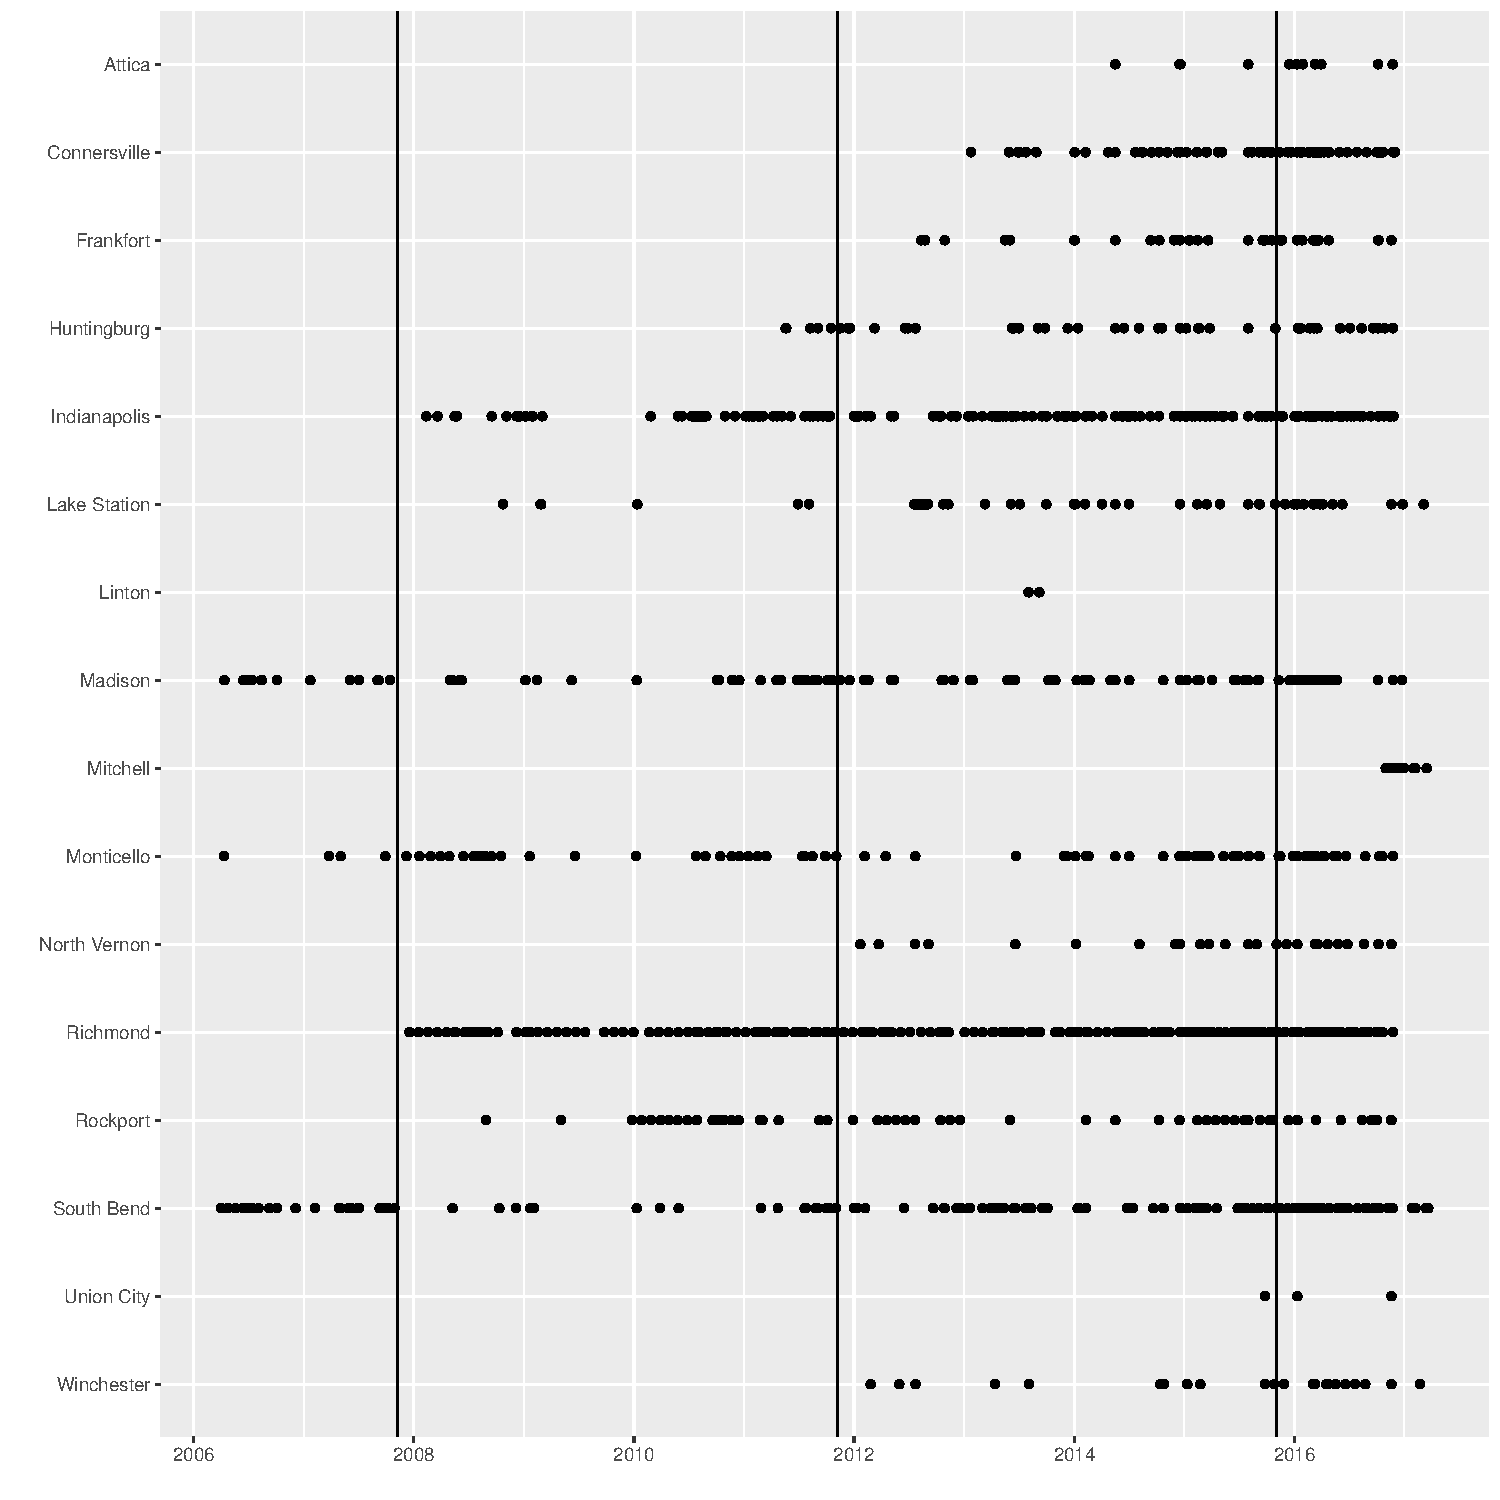
\includegraphics[width=\linewidth]{figures/Snapshots.pdf}
\end{figure}


\begin{figure}[!ht]
	\centering
	%\caption{Population coverage}
	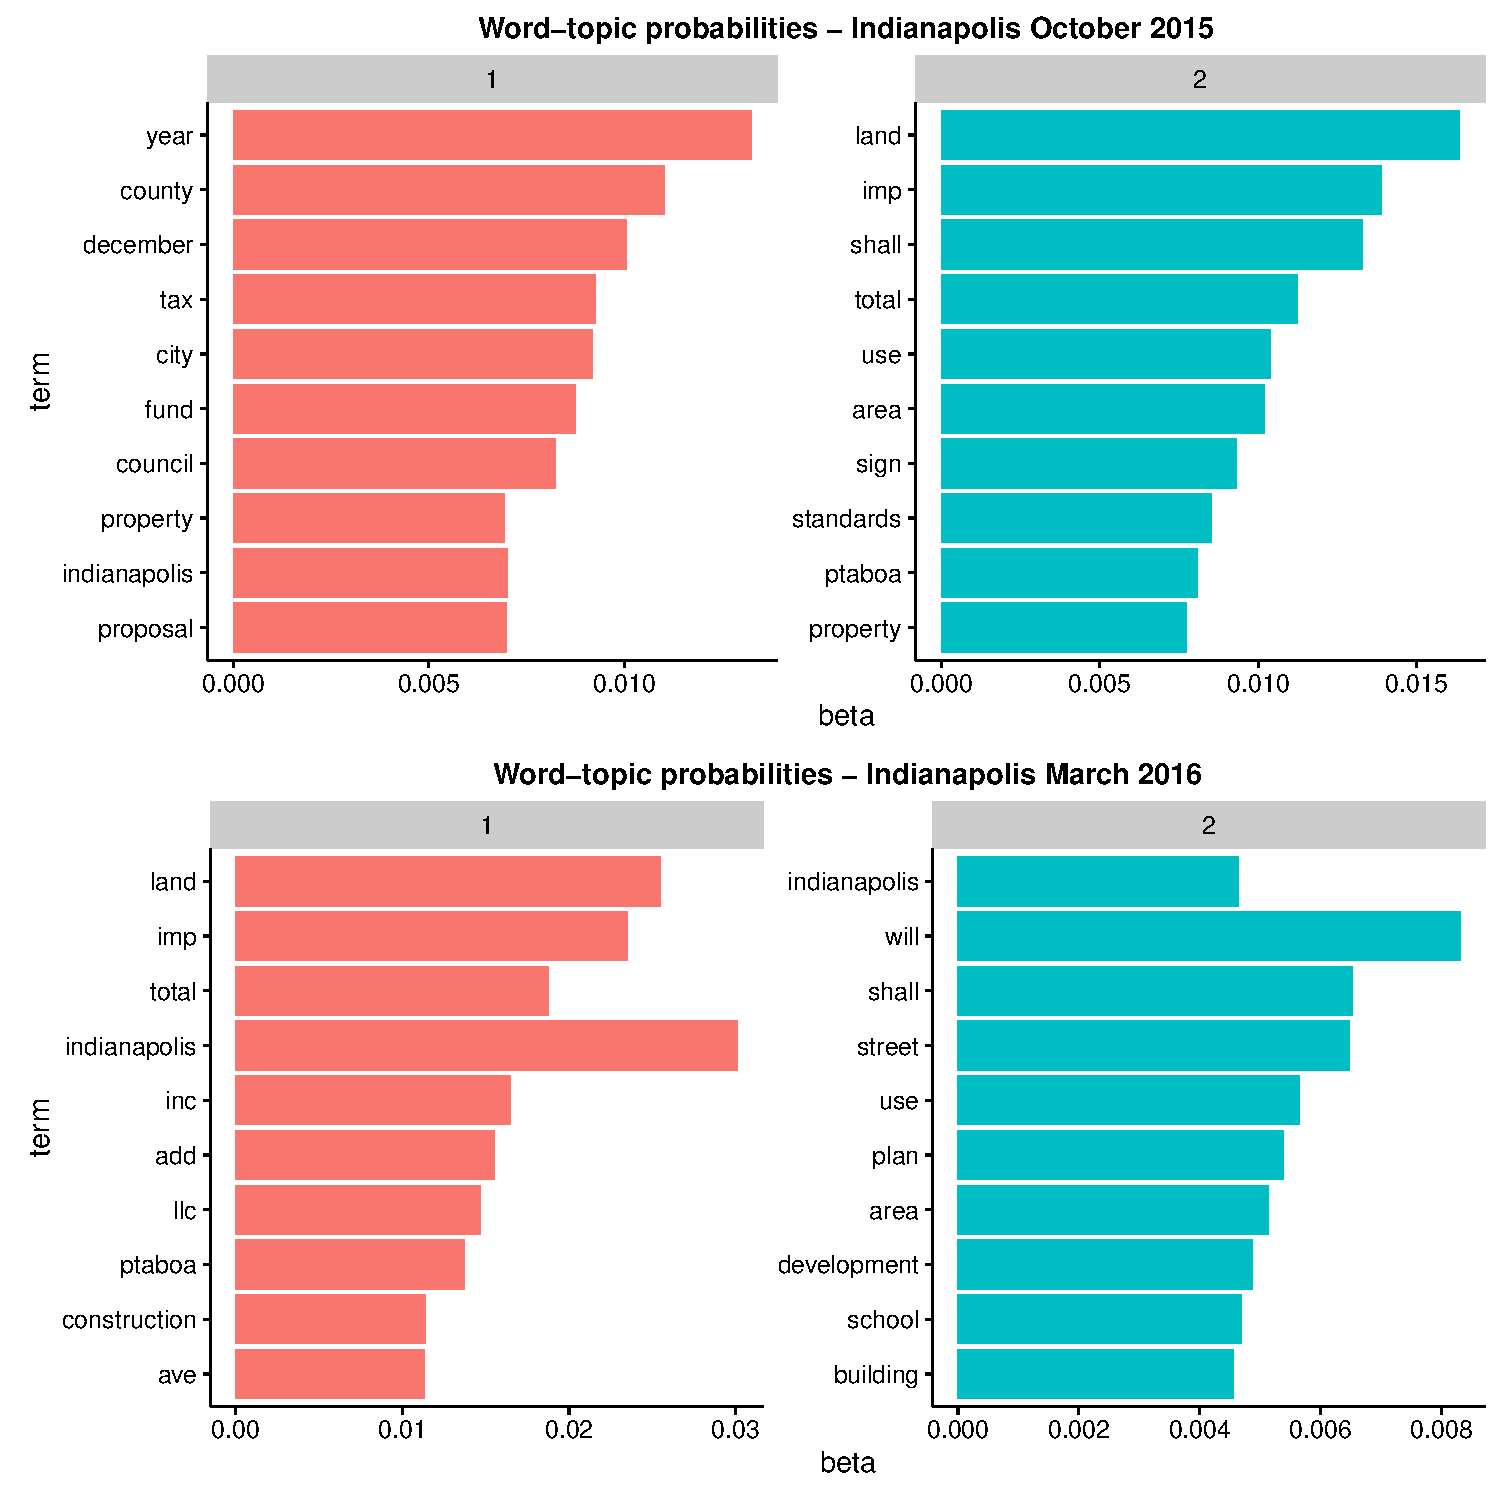
\includegraphics[width=\linewidth]{figures/wtpIndy.pdf}
\end{figure}

% latex table generated in R 3.3.2 by xtable 1.8-2 package
% Fri Mar 24 12:52:43 2017
\begin{table}[ht]
\centering
\begin{tabular}{lrrrr}
  \hline
File type & oct15 & jan16 & feb16 & mar16 \\ 
  \hline
.pdf & 179 & 183 & 111 & 197 \\ 
  .aspx &  99 & 112 & 116 &  76 \\ 
  .jpg &  22 &  24 &  17 &  12 \\ 
  .gif &   3 &   5 &   1 &   5 \\ 
  .JPG &   3 &   2 &   1 &   5 \\ 
  .png &   3 &   7 &   2 &   1 \\ 
  .asmx &   2 &   1 &   1 &   5 \\ 
  .PDF &   1 &   1 &   1 &   2 \\ 
   \hline
\end{tabular}
\caption{File types of Indy.gov at different points in time} 
\end{table}

\newpage

%\bibliographystyle{apsr} % apsr stopped working for me
\bibliographystyle{plainnat}
\bibliography{ref}

\end{document}
